% GNUPLOT: LaTeX picture with Postscript
\begingroup
  \makeatletter
  \providecommand\color[2][]{%
    \GenericError{(gnuplot) \space\space\space\@spaces}{%
      Package color not loaded in conjunction with
      terminal option `colourtext'%
    }{See the gnuplot documentation for explanation.%
    }{Either use 'blacktext' in gnuplot or load the package
      color.sty in LaTeX.}%
    \renewcommand\color[2][]{}%
  }%
  \providecommand\includegraphics[2][]{%
    \GenericError{(gnuplot) \space\space\space\@spaces}{%
      Package graphicx or graphics not loaded%
    }{See the gnuplot documentation for explanation.%
    }{The gnuplot epslatex terminal needs graphicx.sty or graphics.sty.}%
    \renewcommand\includegraphics[2][]{}%
  }%
  \providecommand\rotatebox[2]{#2}%
  \@ifundefined{ifGPcolor}{%
    \newif\ifGPcolor
    \GPcolortrue
  }{}%
  \@ifundefined{ifGPblacktext}{%
    \newif\ifGPblacktext
    \GPblacktexttrue
  }{}%
  % define a \g@addto@macro without @ in the name:
  \let\gplgaddtomacro\g@addto@macro
  % define empty templates for all commands taking text:
  \gdef\gplbacktext{}%
  \gdef\gplfronttext{}%
  \makeatother
  \ifGPblacktext
    % no textcolor at all
    \def\colorrgb#1{}%
    \def\colorgray#1{}%
  \else
    % gray or color?
    \ifGPcolor
      \def\colorrgb#1{\color[rgb]{#1}}%
      \def\colorgray#1{\color[gray]{#1}}%
      \expandafter\def\csname LTw\endcsname{\color{white}}%
      \expandafter\def\csname LTb\endcsname{\color{black}}%
      \expandafter\def\csname LTa\endcsname{\color{black}}%
      \expandafter\def\csname LT0\endcsname{\color[rgb]{1,0,0}}%
      \expandafter\def\csname LT1\endcsname{\color[rgb]{0,1,0}}%
      \expandafter\def\csname LT2\endcsname{\color[rgb]{0,0,1}}%
      \expandafter\def\csname LT3\endcsname{\color[rgb]{1,0,1}}%
      \expandafter\def\csname LT4\endcsname{\color[rgb]{0,1,1}}%
      \expandafter\def\csname LT5\endcsname{\color[rgb]{1,1,0}}%
      \expandafter\def\csname LT6\endcsname{\color[rgb]{0,0,0}}%
      \expandafter\def\csname LT7\endcsname{\color[rgb]{1,0.3,0}}%
      \expandafter\def\csname LT8\endcsname{\color[rgb]{0.5,0.5,0.5}}%
    \else
      % gray
      \def\colorrgb#1{\color{black}}%
      \def\colorgray#1{\color[gray]{#1}}%
      \expandafter\def\csname LTw\endcsname{\color{white}}%
      \expandafter\def\csname LTb\endcsname{\color{black}}%
      \expandafter\def\csname LTa\endcsname{\color{black}}%
      \expandafter\def\csname LT0\endcsname{\color{black}}%
      \expandafter\def\csname LT1\endcsname{\color{black}}%
      \expandafter\def\csname LT2\endcsname{\color{black}}%
      \expandafter\def\csname LT3\endcsname{\color{black}}%
      \expandafter\def\csname LT4\endcsname{\color{black}}%
      \expandafter\def\csname LT5\endcsname{\color{black}}%
      \expandafter\def\csname LT6\endcsname{\color{black}}%
      \expandafter\def\csname LT7\endcsname{\color{black}}%
      \expandafter\def\csname LT8\endcsname{\color{black}}%
    \fi
  \fi
    \setlength{\unitlength}{0.0500bp}%
    \ifx\gptboxheight\undefined%
      \newlength{\gptboxheight}%
      \newlength{\gptboxwidth}%
      \newsavebox{\gptboxtext}%
    \fi%
    \setlength{\fboxrule}{0.5pt}%
    \setlength{\fboxsep}{1pt}%
\begin{picture}(6760.00,4320.00)%
    \gplgaddtomacro\gplbacktext{%
      \csname LTb\endcsname%
      \put(470,508){\makebox(0,0)[r]{\strut{}$0$}}%
      \csname LTb\endcsname%
      \put(470,1175){\makebox(0,0)[r]{\strut{}$2$}}%
      \csname LTb\endcsname%
      \put(470,1842){\makebox(0,0)[r]{\strut{}$4$}}%
      \csname LTb\endcsname%
      \put(470,2508){\makebox(0,0)[r]{\strut{}$6$}}%
      \csname LTb\endcsname%
      \put(470,3175){\makebox(0,0)[r]{\strut{}$8$}}%
      \csname LTb\endcsname%
      \put(470,3842){\makebox(0,0)[r]{\strut{}$10$}}%
      \csname LTb\endcsname%
      \put(695,349){\makebox(0,0){\strut{}$100$}}%
      \csname LTb\endcsname%
      \put(1072,349){\makebox(0,0){\strut{}$200$}}%
      \csname LTb\endcsname%
      \put(1449,349){\makebox(0,0){\strut{}$300$}}%
      \csname LTb\endcsname%
      \put(1827,349){\makebox(0,0){\strut{}$400$}}%
      \csname LTb\endcsname%
      \put(2204,349){\makebox(0,0){\strut{}$500$}}%
      \csname LTb\endcsname%
      \put(2581,349){\makebox(0,0){\strut{}$600$}}%
      \csname LTb\endcsname%
      \put(2959,349){\makebox(0,0){\strut{}$700$}}%
      \csname LTb\endcsname%
      \put(3336,349){\makebox(0,0){\strut{}$800$}}%
      \csname LTb\endcsname%
      \put(3713,349){\makebox(0,0){\strut{}$900$}}%
      \csname LTb\endcsname%
      \put(4091,349){\makebox(0,0){\strut{}$1000$}}%
      \csname LTb\endcsname%
      \put(4468,349){\makebox(0,0){\strut{}$1100$}}%
      \csname LTb\endcsname%
      \put(4845,349){\makebox(0,0){\strut{}$1200$}}%
      \csname LTb\endcsname%
      \put(5222,349){\makebox(0,0){\strut{}$1300$}}%
      \csname LTb\endcsname%
      \put(5600,349){\makebox(0,0){\strut{}$1400$}}%
      \csname LTb\endcsname%
      \put(5977,349){\makebox(0,0){\strut{}$1500$}}%
      \csname LTb\endcsname%
      \put(6066,508){\makebox(0,0)[l]{\strut{}$0$}}%
      \csname LTb\endcsname%
      \put(6066,1175){\makebox(0,0)[l]{\strut{}$2$}}%
      \csname LTb\endcsname%
      \put(6066,1842){\makebox(0,0)[l]{\strut{}$4$}}%
      \csname LTb\endcsname%
      \put(6066,2508){\makebox(0,0)[l]{\strut{}$6$}}%
      \csname LTb\endcsname%
      \put(6066,3175){\makebox(0,0)[l]{\strut{}$8$}}%
      \csname LTb\endcsname%
      \put(6066,3842){\makebox(0,0)[l]{\strut{}$10$}}%
    }%
    \gplgaddtomacro\gplfronttext{%
      \csname LTb\endcsname%
      \put(123,2175){\rotatebox{-270}{\makebox(0,0){\strut{}Loss \%}}}%
      \csname LTb\endcsname%
      \put(6411,2175){\rotatebox{-270}{\makebox(0,0){\strut{}Rate (Gbps)}}}%
      \csname LTb\endcsname%
      \put(3268,111){\makebox(0,0){\strut{}Frame size (bytes)}}%
      \csname LTb\endcsname%
      \put(3268,4081){\makebox(0,0){\strut{}Capture rate}}%
      \csname LTb\endcsname%
      \put(5291,1286){\makebox(0,0)[r]{\strut{}Lost \%}}%
      \csname LTb\endcsname%
      \put(5291,1127){\makebox(0,0)[r]{\strut{}Port Drop \%}}%
      \csname LTb\endcsname%
      \put(5291,968){\makebox(0,0)[r]{\strut{}Send rate}}%
      \csname LTb\endcsname%
      \put(5291,809){\makebox(0,0)[r]{\strut{}Capture rate}}%
      \csname LTb\endcsname%
      \put(5291,650){\makebox(0,0)[r]{\strut{}Theoretical max rate}}%
    }%
    \gplbacktext
    \put(0,0){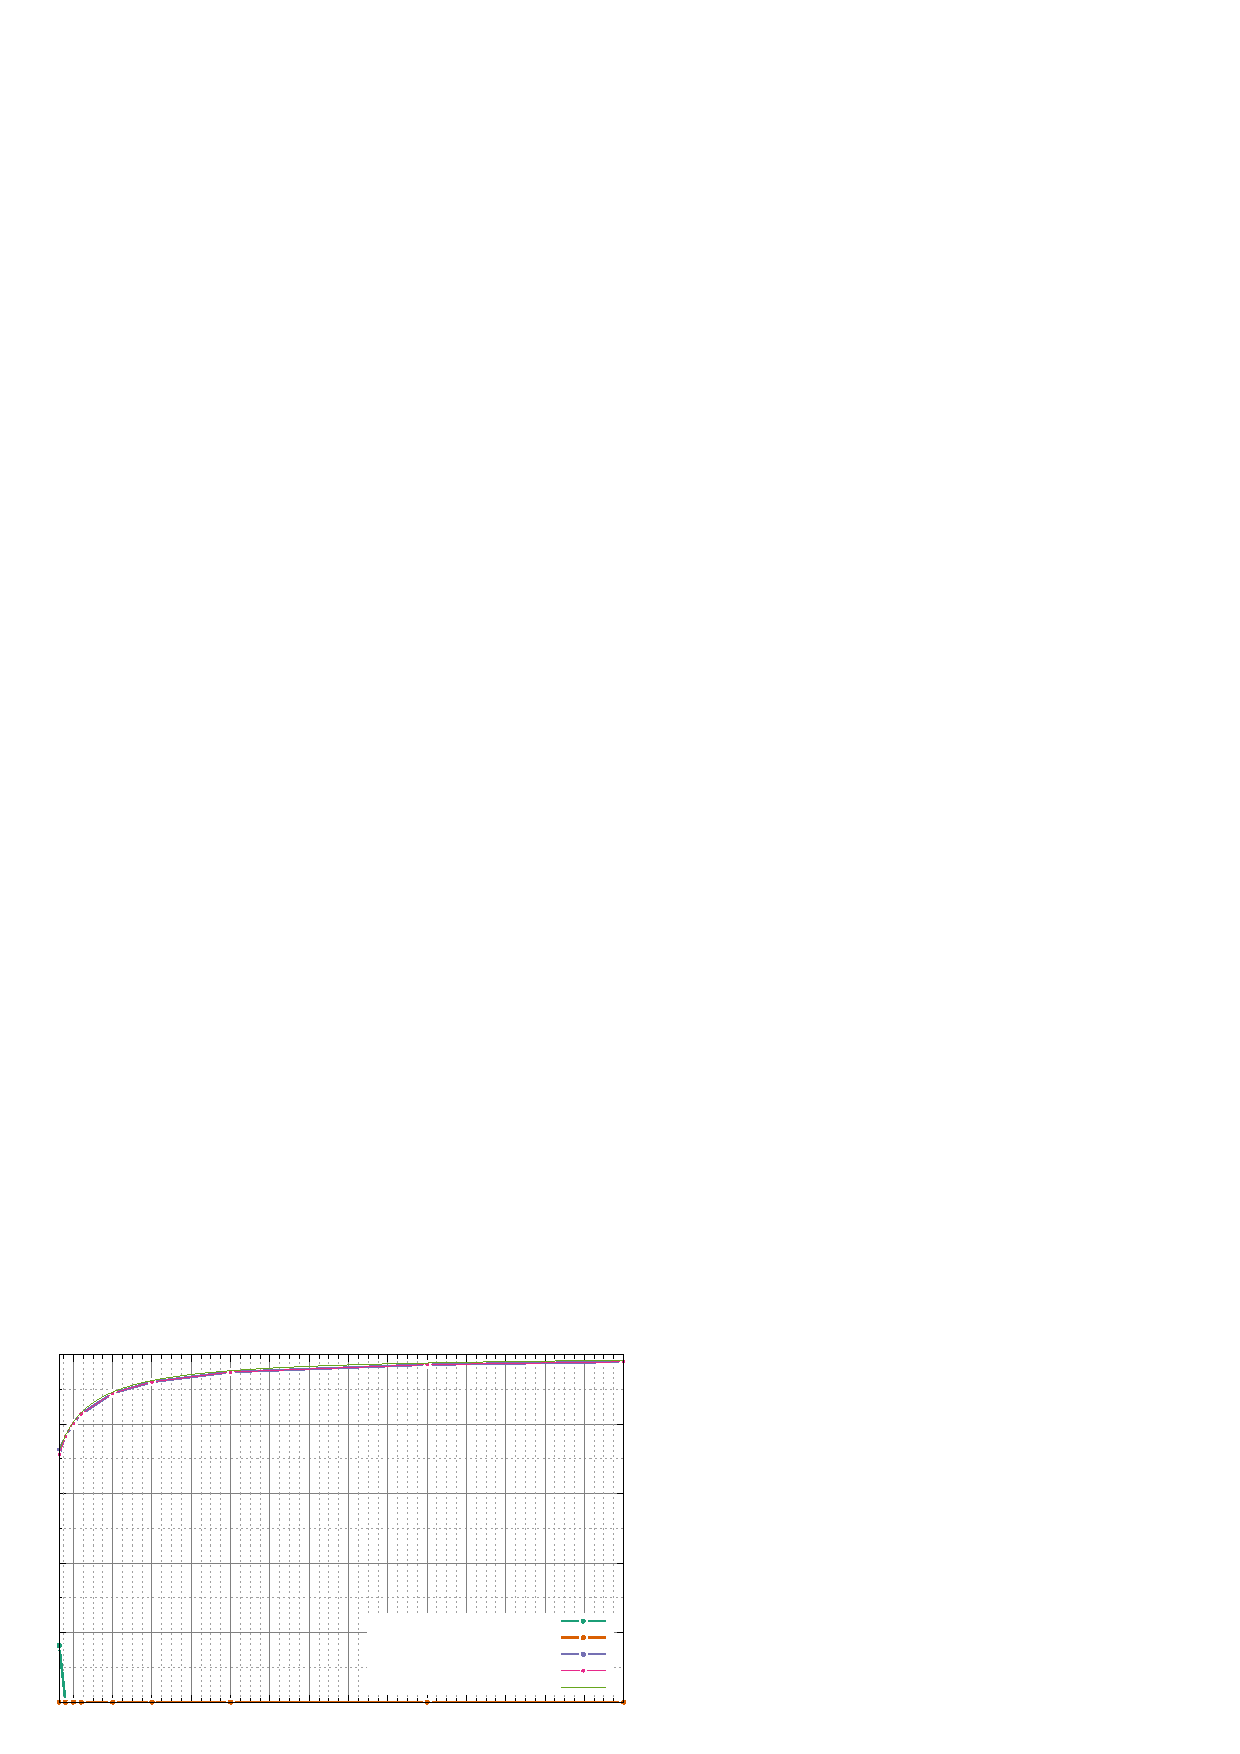
\includegraphics{gnuplot/hpcapdd-nostorage}}%
    \gplfronttext
  \end{picture}%
\endgroup
